\section{Traffic Lights}

	Start by placing the 3 LEDs across the centre of the breadboard, as we did before, and connect each one to a GPIO pin using a jumper cable.

	\begin{center}
		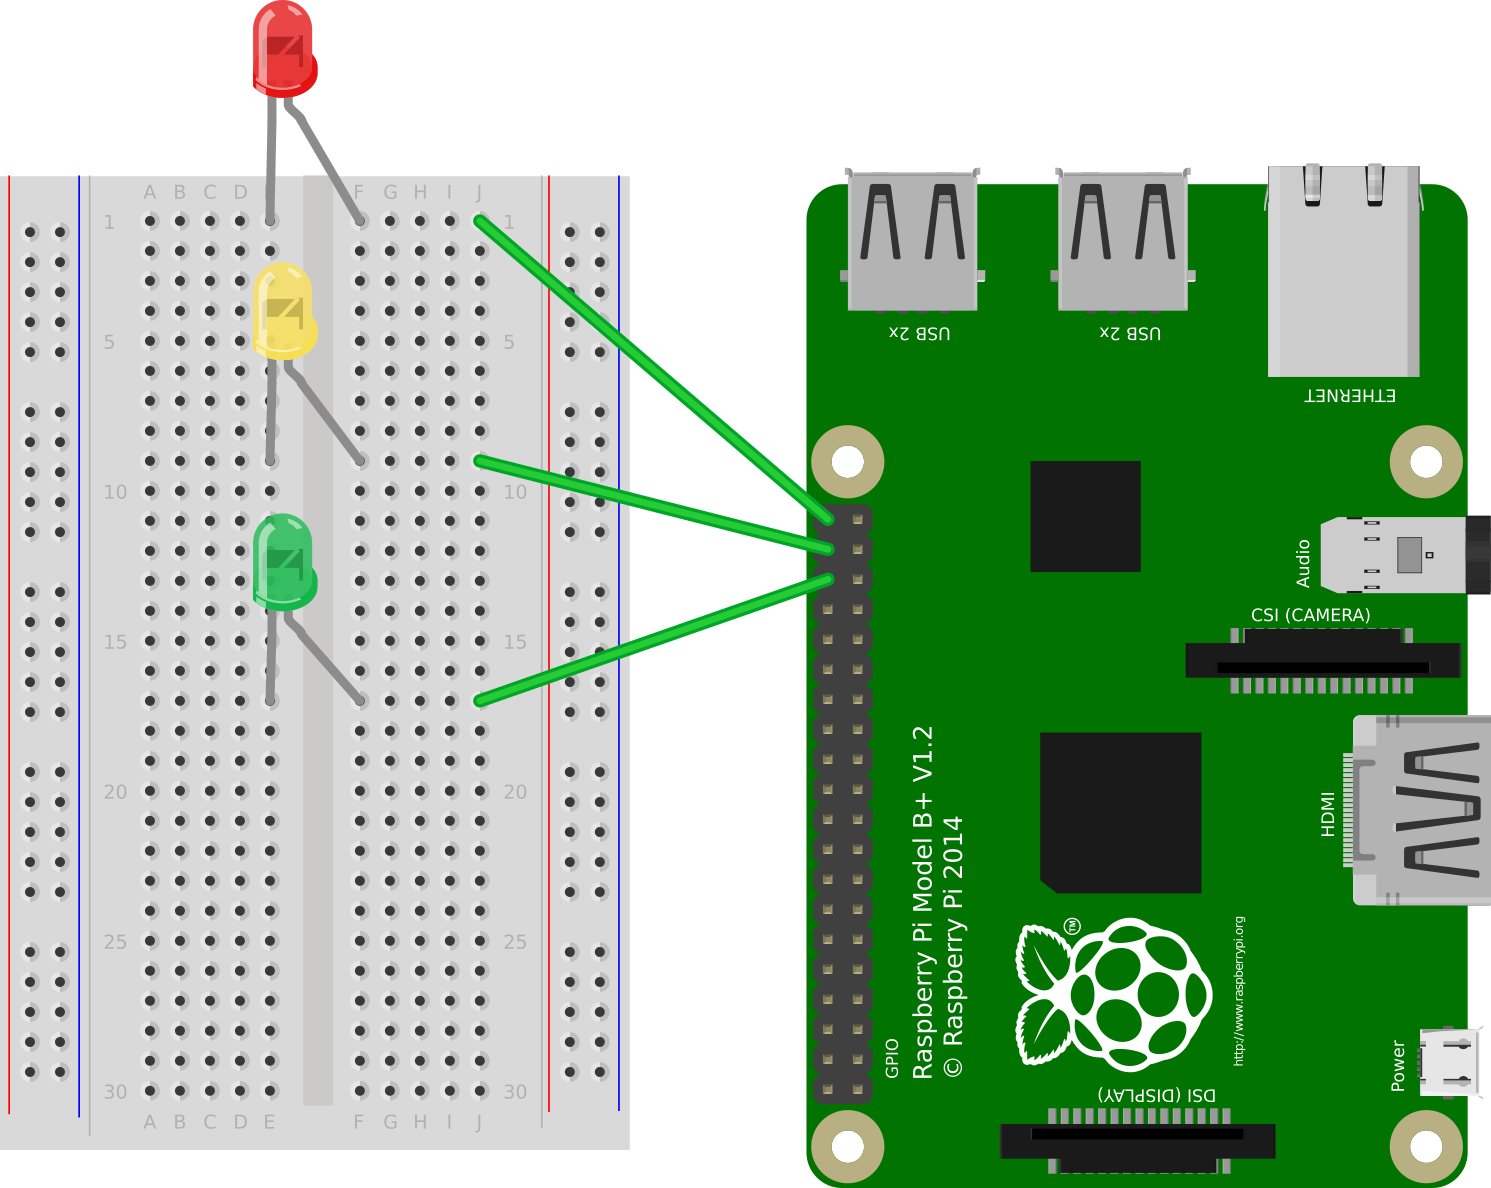
\includegraphics[width=0.7\linewidth]{McrRaspJam/015_GPIOZero/2_trafficlight/2}
	\end{center}

	Each LED still needs a resistor. To save on jumper wires, we'll use the resistors to bridge each LED cathode directly to the negative rail, as shown below.
	
	Then, use a jumper cable to connect the negative rail to a GND pin on the Raspberry Pi.

	\begin{center}
		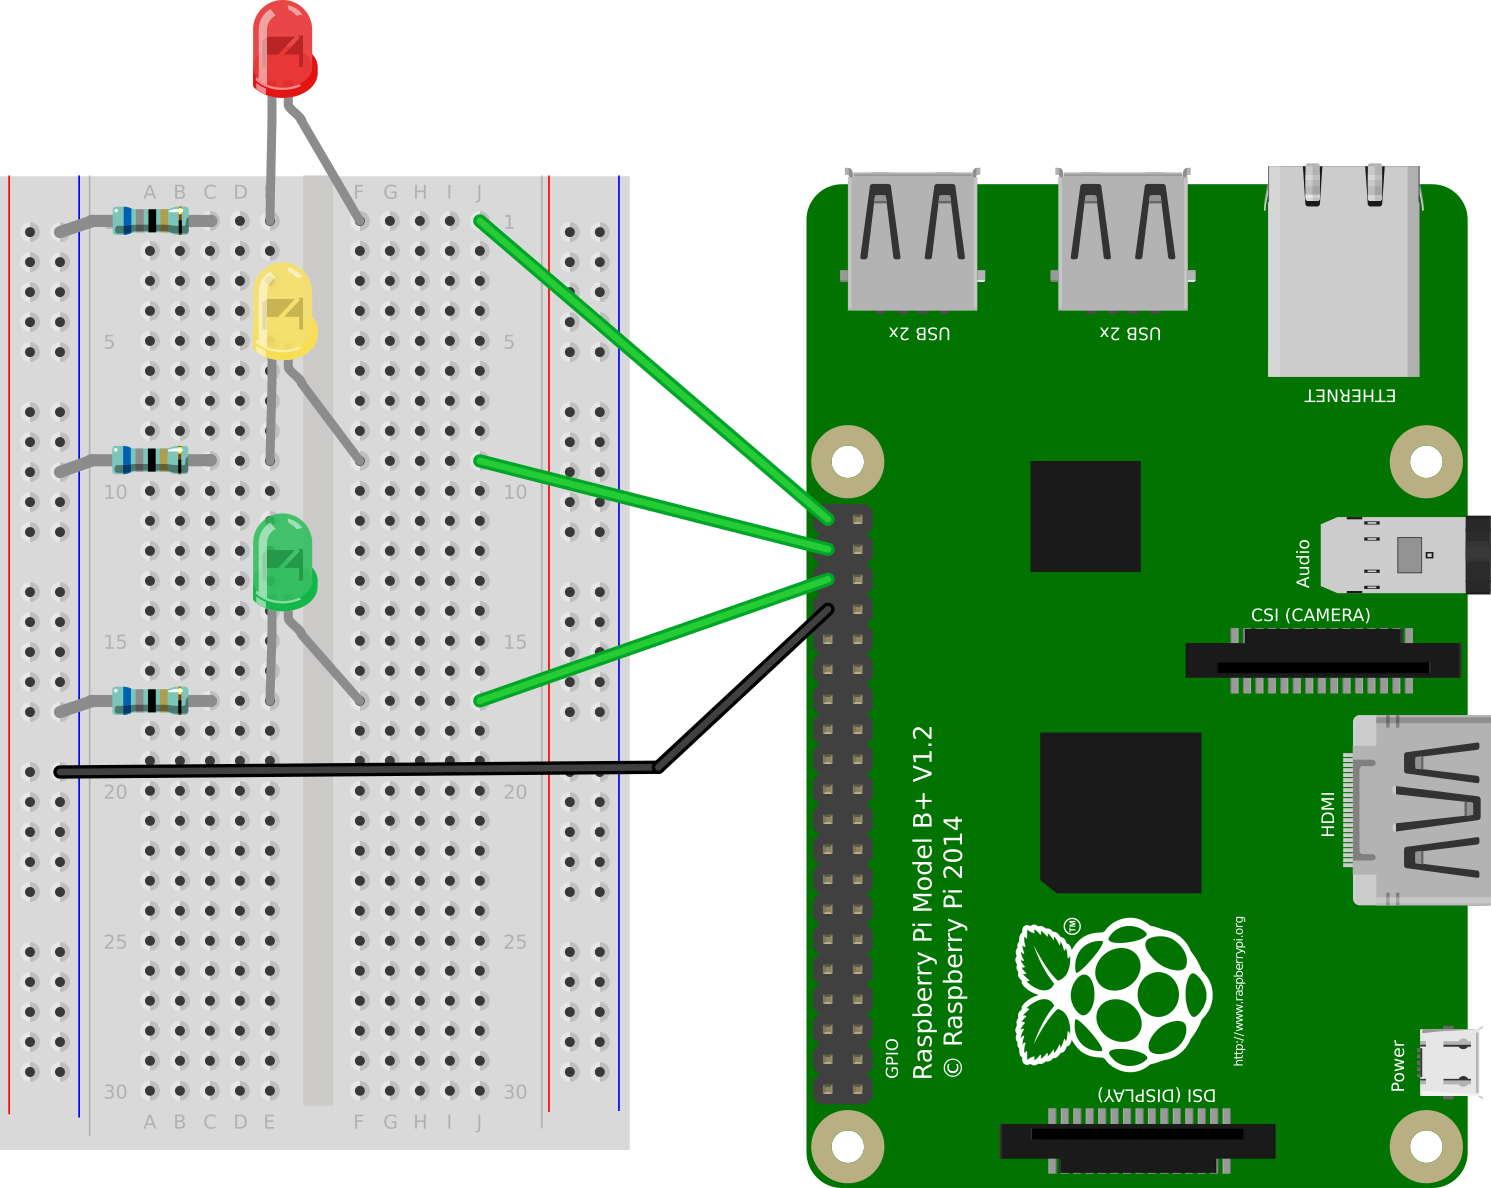
\includegraphics[width=0.7\linewidth]{McrRaspJam/015_GPIOZero/2_trafficlight/3}
	\end{center}

	We'll also place a button on the breadboard in its own circuit. Connect one side of the switch to another GPIO pin, and the other side to a GND pin.

	\begin{center}
		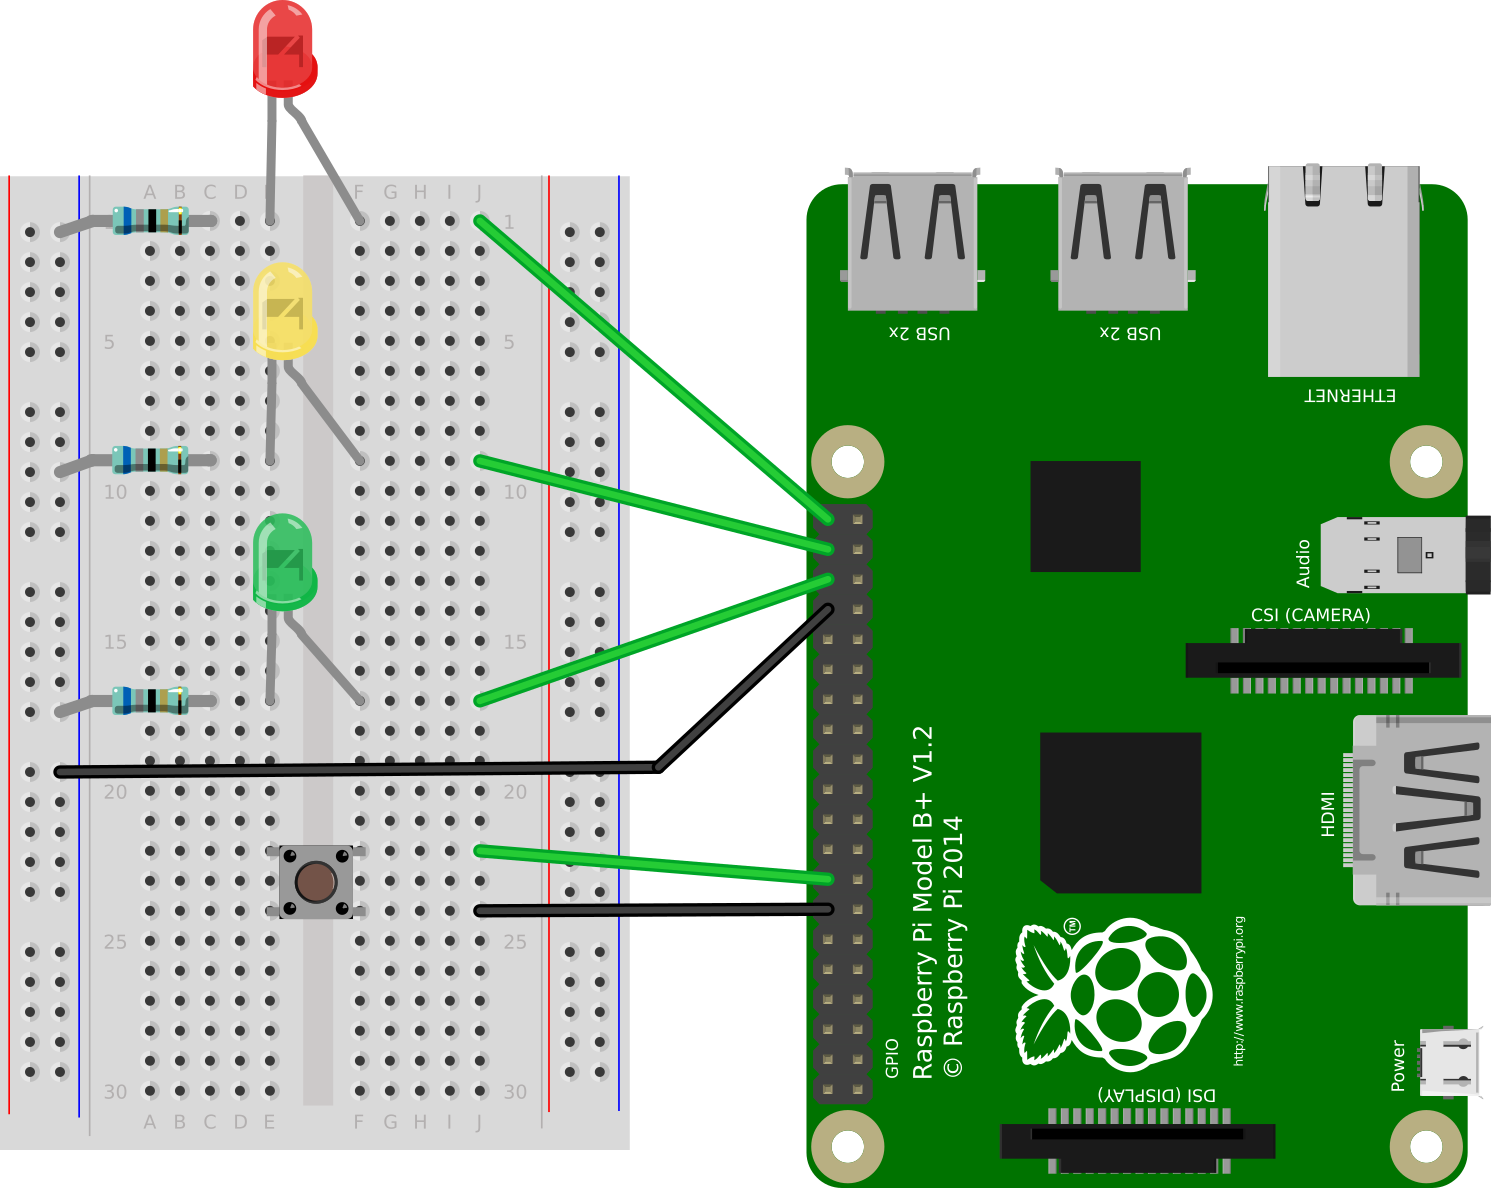
\includegraphics[width=0.7\linewidth]{McrRaspJam/015_GPIOZero/2_trafficlight/4}
	\end{center}

	We now have working circuits for our traffic lights.
	
	\subsection*{Designing the traffic lights}
	
		Now we have a circuit, we need to design how our traffic lights will behave. We'll be designing them as a \textbf{pelican crossing}.
		
		\begin{figure}[h]
			\centering
			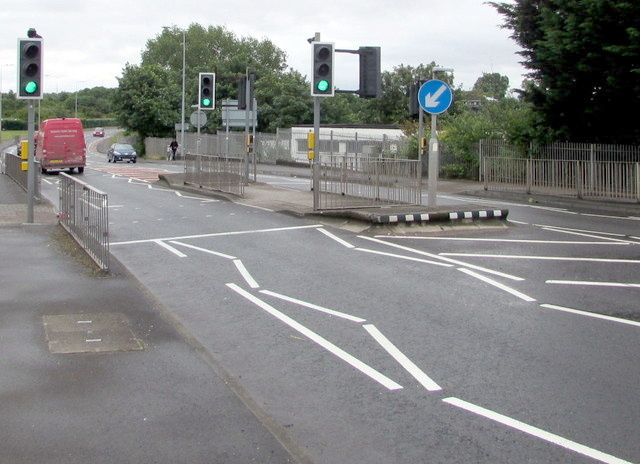
\includegraphics[width=0.5\linewidth]{McrRaspJam/015_GPIOZero/2_trafficlight/pelican}
			\caption{A pelican crossing}
			% From geograph.org.uk
			\label{fig:pelican}
		\end{figure}
		
		Ignoring the button to begin with, we want our traffic lights to stay on green for most of the time, but switch to red occasionally to allow pedestrians to cross.
		
		One tool that is used for these kinds of design problem is a \textit{state transition diagram}. We can use one of these to break down the traffic light sequence into simple steps.
		
		The following is a state transition diagram for a set of traffic lights. The squares are the `states'---in our case the colour of the lights---and the lines are the transitions---the thing that determines when states switch, and to where.
		
		\begin{center}
			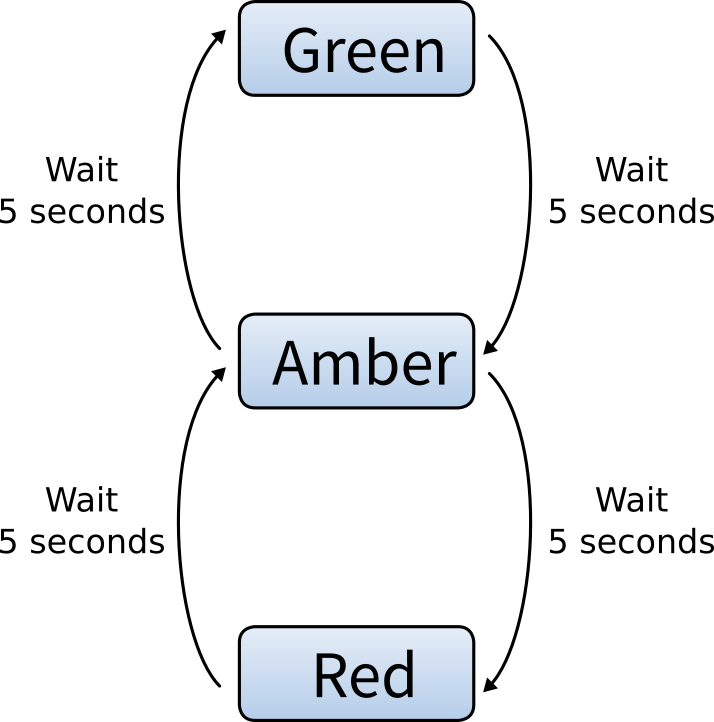
\includegraphics[width=0.6\linewidth]{McrRaspJam/015_GPIOZero/2_trafficlight/transition}
		\end{center}
		
		This state transition diagram isn't very accurate, so you should think of some ways to improve it before you start programming.
		
		\begin{itemize}[noitemsep]
			\item Currently, all of the lights are on for the same amount of time. How long should each transition take?
			\item Are there any times when two lights should be on? (You may need another state)
		\end{itemize}
	
	\subsection*{Programming the traffic lights}
	
		From IDLE, click \mbox{\texttt{File → Open...}} and open \texttt{2\_trafficlight.py}. Fill in the device definitions with the GPIO pins you chose for your circuit. It should look like the following before continuing.
	
		\lstinputlisting[style=Python, lastline=7]{McrRaspJam/015_GPIOZero/2_trafficlight/2_trafficlight.py}
		
		Because our traffic lights run continuously, we'll probably want an infinite loop in our program.
		
		\lstinputlisting[style=Python, firstline=8, firstnumber=8, lastline=9]{McrRaspJam/015_GPIOZero/2_trafficlight/2_trafficlight.py}
		
		We'll start in the `green' state, by turning on that LED, and add the first transition by adding a \texttt{sleep()} delay following this.
		
		\lstinputlisting[style=Python, firstline=10, firstnumber=10, lastline=12]{McrRaspJam/015_GPIOZero/2_trafficlight/2_trafficlight.py}
		
		The rest is up to you, follow this line with the action for your next state, then keep continuing until you have looped back to the starting state.
		
	\subsection*{Adding the button}
	
		Once you're happy with your program so far, you can now implement the pedestrian button.
		
		Start by modifying your state transition diagram. Instead of waiting, one of your transitions will require the button to be pressed.
		
		You can program you button press in a couple of ways. The traditional way of reading GPIO inputs still works:
		
		\lstinputlisting[style=Python, lastline=2]{McrRaspJam/015_GPIOZero/2_trafficlight/button.py}
		
		However, you can also use the function \texttt{wait\_for\_button()}, which is like a \texttt{sleep()} that lasts until the button is pressed.
		
		\lstinputlisting[style=Python, firstline=4]{McrRaspJam/015_GPIOZero/2_trafficlight/button.py}